\section{Date: 2026-08-18}
\noindent \textbf{Series ID: USHSPTLNRSQGSP} 

\noindent This series is titled Quantity Indexes for Real Gross Domestic Product by Industry: Private Industries: Educational Services, Health Care, and Social Assistance: Health Care and Social Assistance: Hospitals and Nursing and Residential Care Facilities for United States (DISCONTINUED) and has a frequency of Annual. The units are Index 2009=100 and the seasonal adjustment is Not Seasonally Adjusted.The observation start date is 1997-01-01 and the observation end date is 2016-01-01.The popularity of this series is 1. \\ 

\noindent \textbf{Series ID: ATNHPIUS35004Q} 

\noindent This series is titled All-Transactions House Price Index for Nassau County-Suffolk County, NY (MSAD) and has a frequency of Quarterly. The units are Index 1995:Q1=100 and the seasonal adjustment is Not Seasonally Adjusted.The observation start date is 1975-07-01 and the observation end date is 2026-01-01.The popularity of this series is 21. \\ 

\subsection{Raw Regression}
\noindent Regresses the two series against each other directly. A significant result here can come just as easily from both series sharing a long-run trend as from any real relationship.

\begin{center}
\begin{tabular}{lclc}
\toprule
\textbf{Dep. Variable:}              & value\_fred\_ATNHPIUS35004Q & \textbf{  R-squared:         } &     0.595   \\
\textbf{Model:}                      &             OLS             & \textbf{  Adj. R-squared:    } &     0.573   \\
\textbf{Method:}                     &        Least Squares        & \textbf{  F-statistic:       } &     26.47   \\
\textbf{Date:}                       &       Tue, 18 Aug 2026      & \textbf{  Prob (F-statistic):} &  6.80e-05   \\
\textbf{Time:}                       &           12:24:41          & \textbf{  Log-Likelihood:    } &   -101.38   \\
\textbf{No. Observations:}           &                20           & \textbf{  AIC:               } &     206.8   \\
\textbf{Df Residuals:}               &                18           & \textbf{  BIC:               } &     208.7   \\
\textbf{Df Model:}                   &                 1           & \textbf{                     } &             \\
\textbf{Covariance Type:}            &          nonrobust          & \textbf{                     } &             \\
\bottomrule
\end{tabular}
\begin{tabular}{lcccccc}
                                     & \textbf{coef} & \textbf{std err} & \textbf{t} & \textbf{P$> |$t$|$} & \textbf{[0.025} & \textbf{0.975]}  \\
\midrule
\textbf{const}                       &    -202.2530  &       81.976     &    -2.467  &         0.024        &     -374.478    &      -30.028     \\
\textbf{value\_fred\_USHSPTLNRSQGSP} &       4.5554  &        0.885     &     5.145  &         0.000        &        2.695    &        6.416     \\
\bottomrule
\end{tabular}
\begin{tabular}{lclc}
\textbf{Omnibus:}       &  3.374 & \textbf{  Durbin-Watson:     } &    0.176  \\
\textbf{Prob(Omnibus):} &  0.185 & \textbf{  Jarque-Bera (JB):  } &    2.734  \\
\textbf{Skew:}          &  0.872 & \textbf{  Prob(JB):          } &    0.255  \\
\textbf{Kurtosis:}      &  2.515 & \textbf{  Cond. No.          } &     837.  \\
\bottomrule
\end{tabular}
%\caption{OLS Regression Results}
\end{center}

Notes: \newline
 [1] Standard Errors assume that the covariance matrix of the errors is correctly specified.

\begin{figure}
\centering
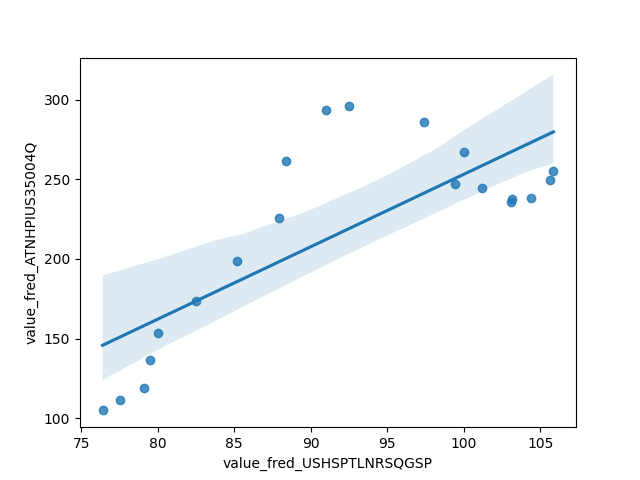
\includegraphics[scale = 0.9]{plots/plot_2026-08-18.png}
\caption{Raw Regression Plot for 2026-08-18}
\end{figure}
\newpage
\subsection{Detrended Regression}
\noindent Regresses the residuals of each series after removing its own linear time trend, so a shared trend can no longer drive the result on its own. A relationship that stays significant here is better evidence of a genuine link between the two series.

\begin{center}
\begin{tabular}{lclc}
\toprule
\textbf{Dep. Variable:}                         & value\_fred\_ATNHPIUS35004Q\_detrended & \textbf{  R-squared:         } &     0.079   \\
\textbf{Model:}                                 &                  OLS                   & \textbf{  Adj. R-squared:    } &     0.028   \\
\textbf{Method:}                                &             Least Squares              & \textbf{  F-statistic:       } &     1.551   \\
\textbf{Date:}                                  &            Tue, 18 Aug 2026            & \textbf{  Prob (F-statistic):} &    0.229    \\
\textbf{Time:}                                  &                12:24:41                & \textbf{  Log-Likelihood:    } &   -101.26   \\
\textbf{No. Observations:}                      &                     20                 & \textbf{  AIC:               } &     206.5   \\
\textbf{Df Residuals:}                          &                     18                 & \textbf{  BIC:               } &     208.5   \\
\textbf{Df Model:}                              &                      1                 & \textbf{                     } &             \\
\textbf{Covariance Type:}                       &               nonrobust                & \textbf{                     } &             \\
\bottomrule
\end{tabular}
\begin{tabular}{lcccccc}
                                                & \textbf{coef} & \textbf{std err} & \textbf{t} & \textbf{P$> |$t$|$} & \textbf{[0.025} & \textbf{0.975]}  \\
\midrule
\textbf{const}                                  &    1.868e-11  &        9.015     &  2.07e-12  &         1.000        &      -18.941    &       18.941     \\
\textbf{value\_fred\_USHSPTLNRSQGSP\_detrended} &       7.1907  &        5.773     &     1.246  &         0.229        &       -4.938    &       19.320     \\
\bottomrule
\end{tabular}
\begin{tabular}{lclc}
\textbf{Omnibus:}       &  3.498 & \textbf{  Durbin-Watson:     } &    0.209  \\
\textbf{Prob(Omnibus):} &  0.174 & \textbf{  Jarque-Bera (JB):  } &    2.716  \\
\textbf{Skew:}          &  0.887 & \textbf{  Prob(JB):          } &    0.257  \\
\textbf{Kurtosis:}      &  2.669 & \textbf{  Cond. No.          } &     1.56  \\
\bottomrule
\end{tabular}
%\caption{OLS Regression Results}
\end{center}

Notes: \newline
 [1] Standard Errors assume that the covariance matrix of the errors is correctly specified.

\begin{figure}
\centering
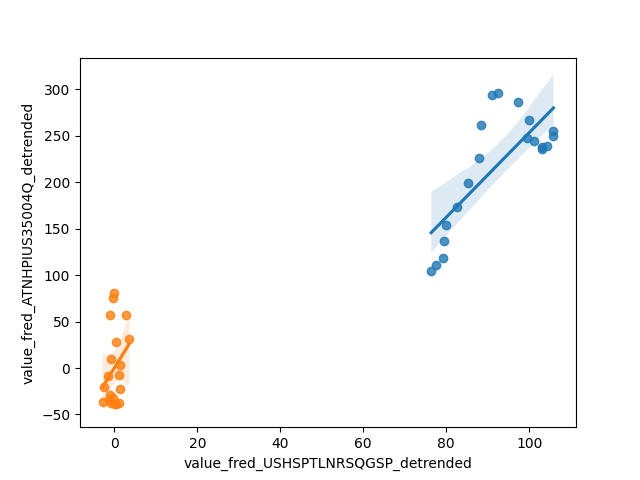
\includegraphics[scale = 0.9]{plots/plot_2026-08-18_detrended.png}
\caption{Detrended Regression Plot for 2026-08-18}
\end{figure}
\newpage
